\section[1]{Introduction}

\begin{frame}{Context}
	Web 2.0
		\begin{itemize}
			\item High data volumes
			\item Dynamic behaviour of the data flow
		\end{itemize}
	
	\begin{figure}
    	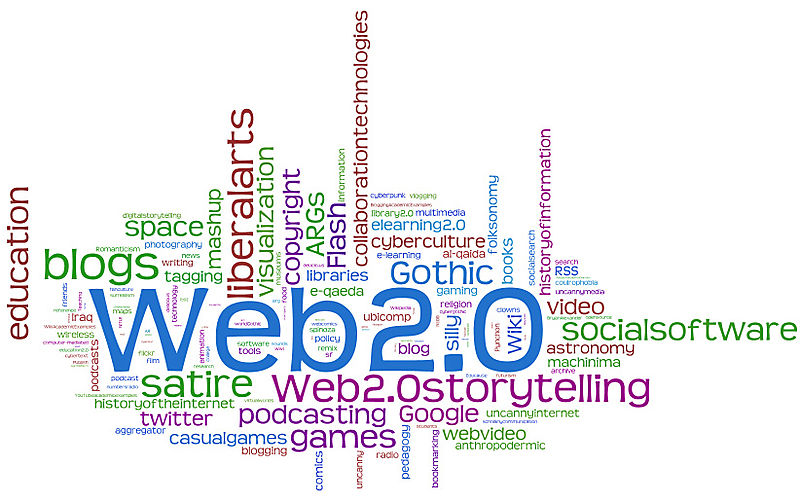
\includegraphics[width=0.6\textwidth]{images/problems/Web.jpg}
    \end{figure}
\end{frame}

\begin{frame}{Context}
		\begin{itemize}
			\item Real-time processing of large data streams
			\begin{itemize}
				\item Low-latency processing
			\end{itemize}
		\end{itemize}
	
		Applications
		\begin{itemize}
			\item Stock exchange prediction
			\item Network security monitoring
			\item Collecting information in natural disasters
		\end{itemize}
\end{frame}

\begin{frame}{Stream processing systems (SPS)}
	Logical architecture
		\begin{itemize}
    		\item The DAG defines the processing logic of the SPS
    		\item A vertex represents a processing operator
    		\item Unidirectional edges represent the data flow
		\end{itemize}
    
    \begin{figure}
		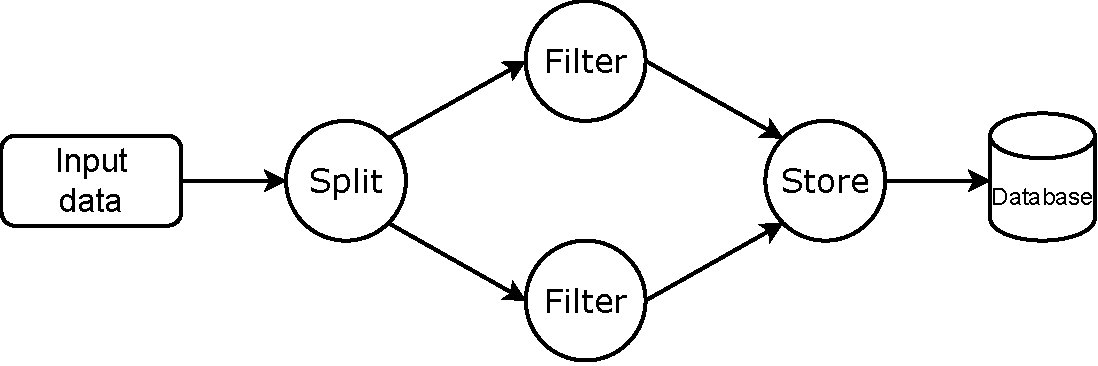
\includegraphics[width=0.75\textwidth]{images/problems/SPS-Concept.pdf}
	\end{figure}
\end{frame}

\begin{frame}{Stream processing systems (SPS)}
	Physical architecture
		\begin{itemize}
    		\item The DAG  must be mapped to a physical environment
    		\item Distributed platform : Cluster or Cloud
		\end{itemize}
	
	\begin{figure}
		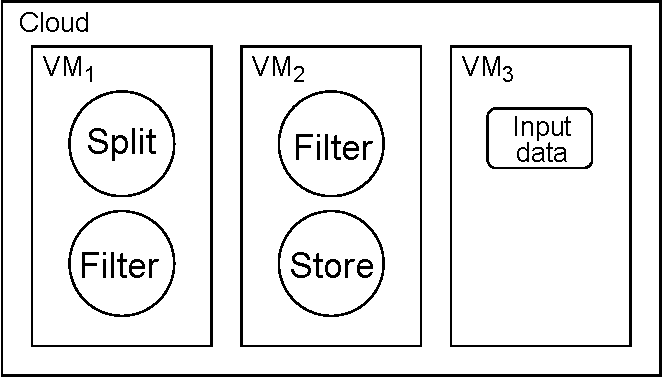
\includegraphics[width=0.5\textwidth]{images/problems/SPS-Physical.pdf}
	\end{figure}
\end{frame}

\begin{frame}{Existing SPS}
	Input rate can present traffic spikes or peaks

	\begin{figure}
		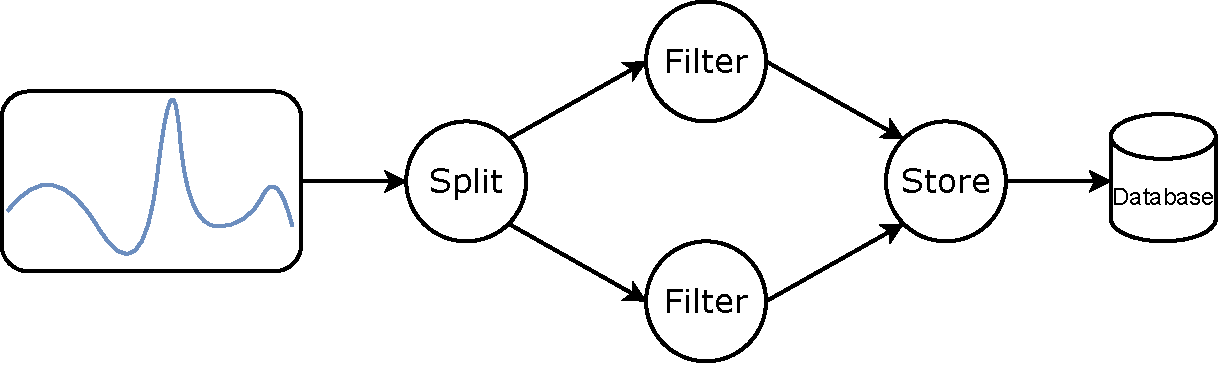
\includegraphics[width=0.65\textwidth]{images/problems/SPS-DynamicDataFlow.pdf}
	\end{figure}
	
	\pause
	
	\begin{alertblock}{Situation}
 	 Overloaded operators and increased end-to-end latency
	\end{alertblock}
\end{frame}

\begin{frame}{Existing SPS}
	Existing SPS Frameworks: 
	\begin{itemize}
		\item Apache Storm [\cite{toshniwal2014storm}]
   		\item Apache Flink [\cite{CarboneKEMHT15}]
	\end{itemize}
    
    \begin{figure}
		
\includegraphics[width=0.4\textwidth]{images/problems/SPS-Framework.png}
	\end{figure}
\end{frame}

\begin{frame}{Existing SPS}
	Replication : Operators can be parallelised
   
    \begin{figure}
		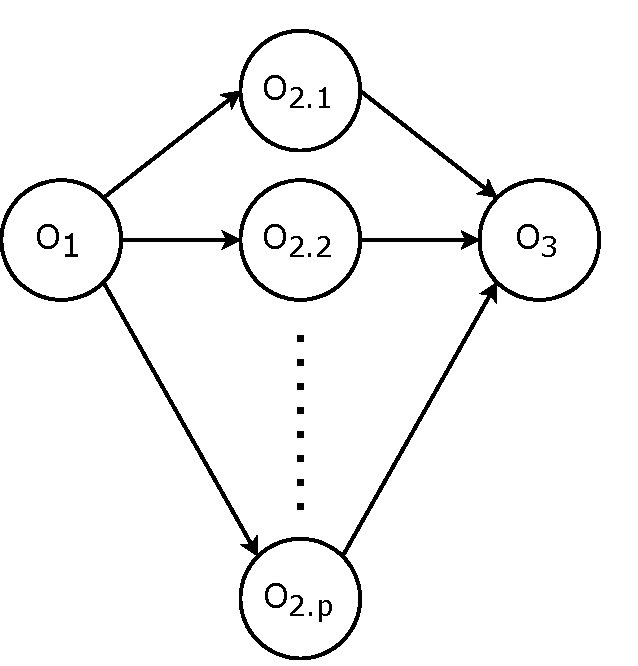
\includegraphics[width=0.35\textwidth]{images/problems/SPS-Operator-Parallelism-Logical.pdf}
	\end{figure}
	
	\pause
	
	\begin{alertblock}{Situation}
		Overprovisioning or underprovisioning of replicas
	\end{alertblock}
\end{frame}



\begin{frame}{Existing SPS}
	\begin{alertblock}{Problem}
		\begin{itemize}
			%\item In general, SPS can present significant fluctuation (peak) in input rate.
		    \item Majority SPSs do not dynamically adapt the number of replicas according to input rate
		\end{itemize}
	\end{alertblock}
	\pause
	\begin{block}{Solution}
		Automatically increase/decrease the number of replicas of critical operators
	\end{block}
\end{frame}
